% 2006 湖南理科 Q18：共用正方形底面 ABCD 的两个正四棱锥。
% 依据固定原卷 PDF 第 1 页。空间位置仅为示意，未按比例绘制。
% 原图可辨线型：底面 DA、DC，棱 PD、QD，以及 P/O/Q 的竖向投影线为虚线；
% 底面 AB、BC 与其余锥棱为实线。底面中心 O 只作投影辅助点，原图未标字母。
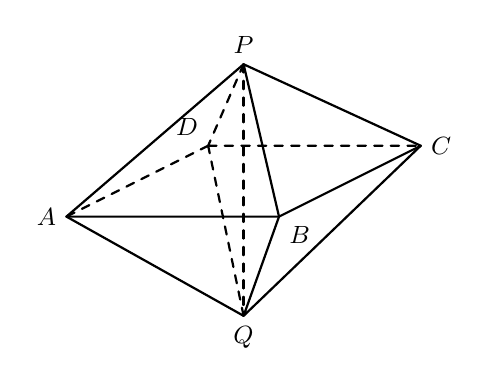
\begin{tikzpicture}[x=0.9cm,y=0.9cm,line cap=round,line join=round,
                    line width=0.8pt,font=\small]
  % 底面顶点按原图的投影次序放置；O 为未标记的底面中心。
  \coordinate (A) at (-2,0);
  \coordinate (B) at (1,0);
  \coordinate (C) at (3,1);
  \coordinate (D) at (0,1);
  \coordinate (O) at (0.5,0.5);
  \coordinate (P) at (0.5,2.15);
  \coordinate (Q) at (0.5,-1.4);

  % 原图以虚线表示的后侧底棱、后侧锥棱和两条高的投影。
  \draw[dashed] (D)--(A) (D)--(C) (P)--(D) (Q)--(D);
  \draw[dashed] (P)--(O)--(Q);

  % 原图其余可见底棱与锥棱。
  \draw (A)--(B)--(C);
  \draw (P)--(A) (P)--(B) (P)--(C);
  \draw (Q)--(A) (Q)--(B) (Q)--(C);

  \node[above] at (P) {$P$};
  \node[below] at (Q) {$Q$};
  \node[left] at (A) {$A$};
  \node[below right] at (B) {$B$};
  \node[right] at (C) {$C$};
  \node[above left] at (D) {$D$};
\end{tikzpicture}
